\section{Aufbau der Benutzeroberfläche}
Die Benutzeroberfläche kann als Web-App direkt zum Homebildschirm eines mobilen Endgeräts hinzugefügt werden.  
Dadurch lässt sich die Steuerung der WordClock ähnlich wie eine native Smartphone-Anwendung bedienen (vgl. Abb.~\ref{fig:APIHomebildschirm}).

\begin{figure}[H]
    \centering
    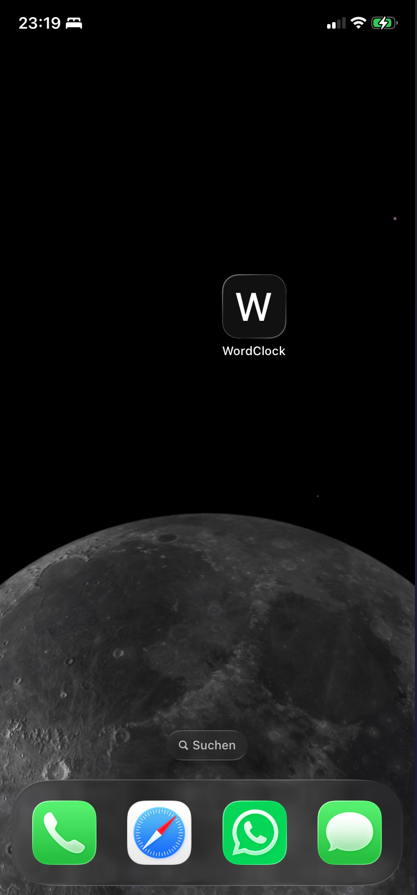
\includegraphics[width=0.37\linewidth]{inhalt/bilder/APIHomebildschirm.png}
    \caption[Die HTML-UI als Web-App auf dem Homebildschirm]{Die \gls{html}-\gls{ui} der WordClock kann als Web-App zum Homebildschirm hinzugefügt werden und ermöglicht damit einen schnellen Zugriff auf diese.}
    \label{fig:APIHomebildschirm}
\end{figure}

Nach dem Öffnen der Benutzeroberfläche werden im ersten Segment: „Anzeige“ die aktuellen Statusinformationen der WordClock angezeigt.  
Hierzu zählen unter anderem Uhrzeit, Wetterdaten, Helligkeit, Farbwerte sowie Sensorinformationen (vgl. Abb.~\ref{fig:APIParameteruebersicht}).

\begin{figure}[H]
    \centering
    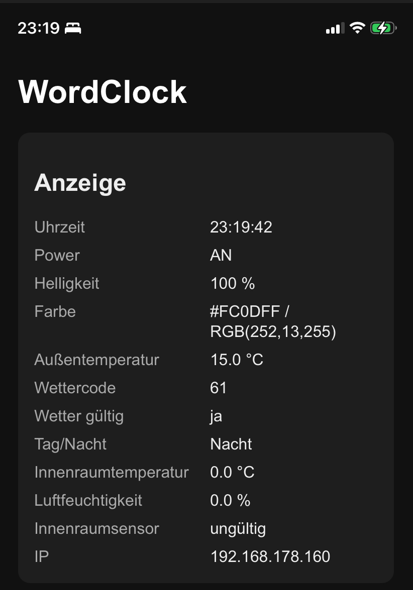
\includegraphics[width=0.5\textwidth]{inhalt/bilder/APIParameterübersicht.png}
    \caption{Übersicht der aktuellen Systemparameter und Statusinformationen.}
    \label{fig:APIParameteruebersicht}
\end{figure}

Im Segement: „Steuerung“ der Benutzeroberfläche befinden sich die Bedienelemente.  
Über diese kann die WordClock ein- und ausgeschaltet sowie eine manuelle Aktualisierung der Wetterdaten ausgelöst werden (vgl. Abb.~\ref{fig:APIFarbe1}).
Im dritten Segement: „Farbe/Helligkeit“ kann die Farbe und die Helligkeit der \gls{led}-Beleuchtung angepasst werden.  
Die Helligkeit wird über einen Slider eingestellt (vgl. Abb.~\ref{fig:APIFarbe1}).
Die Farbe kann z.B. über eine Spektrums-Schaltfläche ausgewählt werden.
Diese öffnet sich wenn man auf die aktuell im Segment angezeigte Farbe drückt (vgl. Abb.~\ref{fig:APIFarbe2}).
Die Änderungen werden mit der Schaltfläche  „Speichern“ übernommen (vgl. Abb.~\ref{fig:APIFarbe1}).

\begin{figure}[H]
  \centering
	\begin{subfigure}{0.45\textwidth}
      \centering
      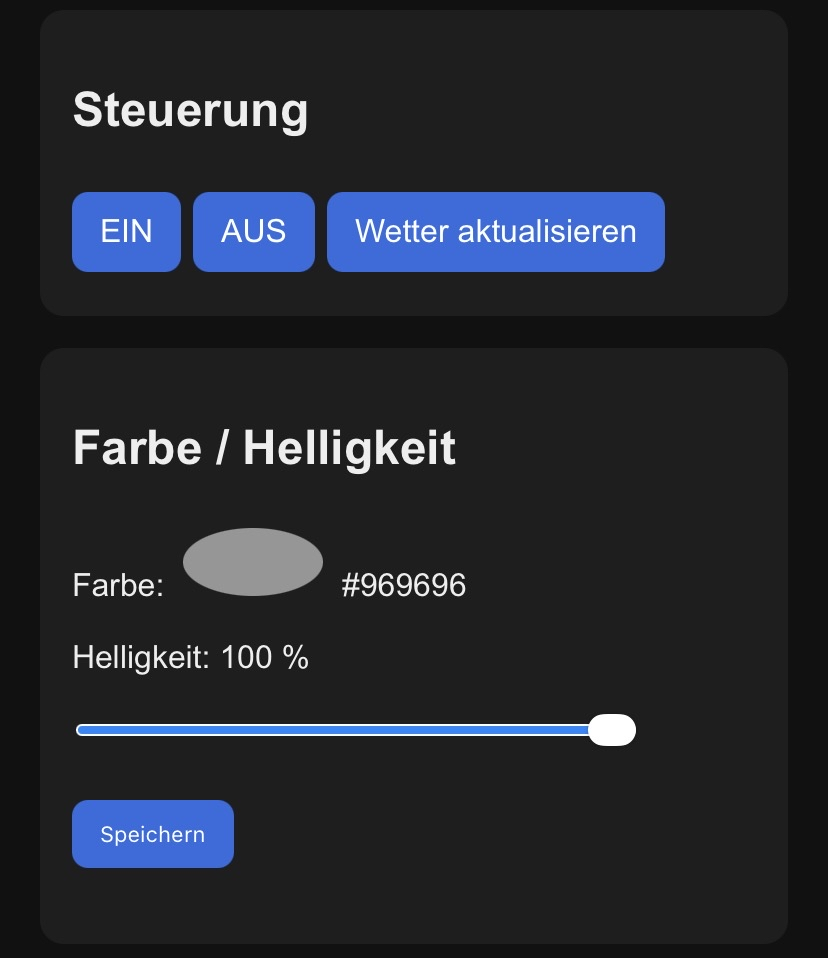
\includegraphics[width=\textwidth]{inhalt/bilder/APIFarbe1.png}
      \caption{Segment drei der \gls{ui} mit einem Slider für die Helligkeit und einer Schaltfläche zur Auswahl der Farbe für die \gls{led}-Beleuchtung.}
      \label{fig:APIFarbe1}
	\end{subfigure}
	\\%\hfill
	\begin{subfigure}{0.45\textwidth}
      \centering
      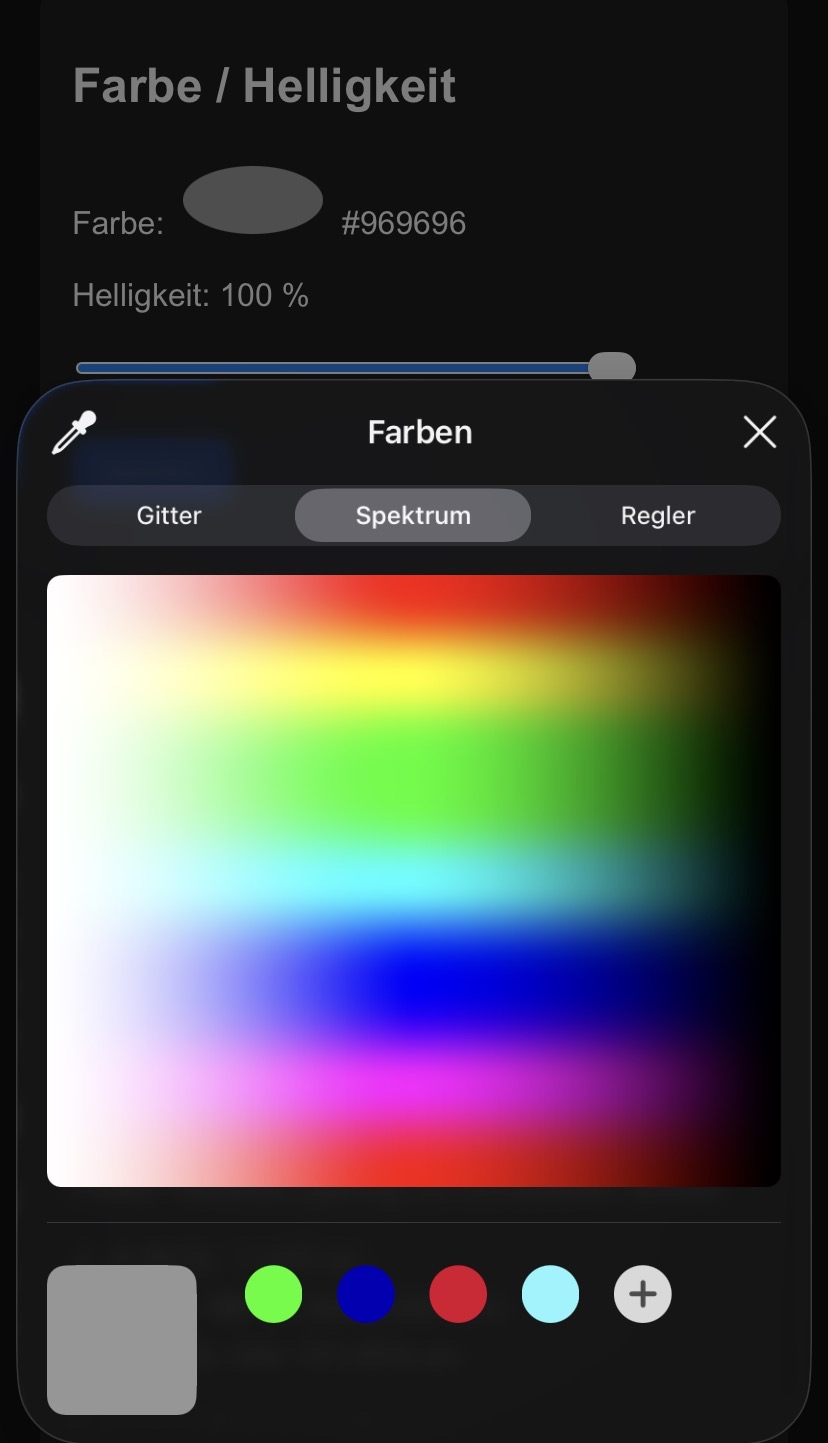
\includegraphics[width=\textwidth]{inhalt/bilder/APIFarbe2.png}
      \caption{Einstellmöglichkeiten für die Farbe der \gls{led}-Beleuchtung mit der Möglichkeit Favoriten zu speichern.}
      \label{fig:APIFarbe2}
	\end{subfigure}
	\caption{Farb- und Helligkeitseinstellungen in der \gls{ui}.}
\end{figure}

Das vierte Segment: „Skalen- \& Sensor-Erklärung“ listet die vier informativen Zusatzfunktionen der WordClock auf und erläutert, unter welchen Bedingungen die verschiedenen Funktionen welche Anzeige liefern (vgl. Abb.~\ref{fig:AnzeigeErklaerung}).

\begin{figure}[H]
    \centering
    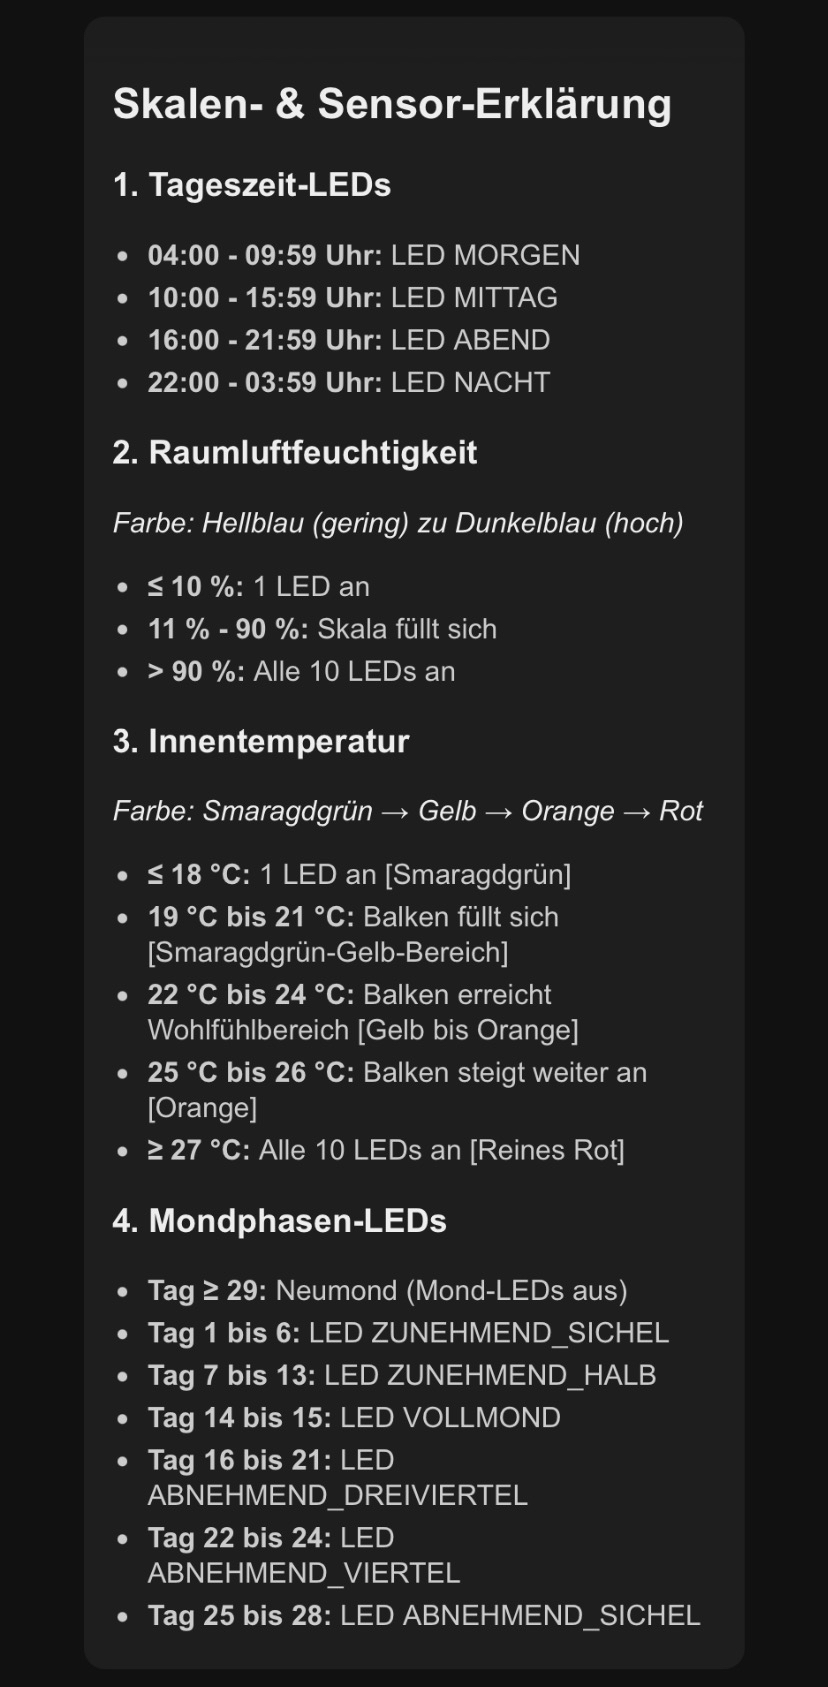
\includegraphics[width=0.55\textwidth]{inhalt/bilder/SkalenSensor.png}
    \caption{Erklärung der Anzeigeoptionen für die vier informativen Zusatzfunktionen.}
    \label{fig:AnzeigeErklaerung}
\end{figure}

Im letzten Segment: „API“ kann man das \gls{json}-Statusfile aufrufen, das die Werte für die Oberfläche bereitstellt und in dem die genauen Variablennamen aufgeführt sind (vgl. Abb.~\ref{fig:Json}).

\begin{figure}[H]
  \centering
	\begin{subfigure}{0.55\textwidth}
      \centering
      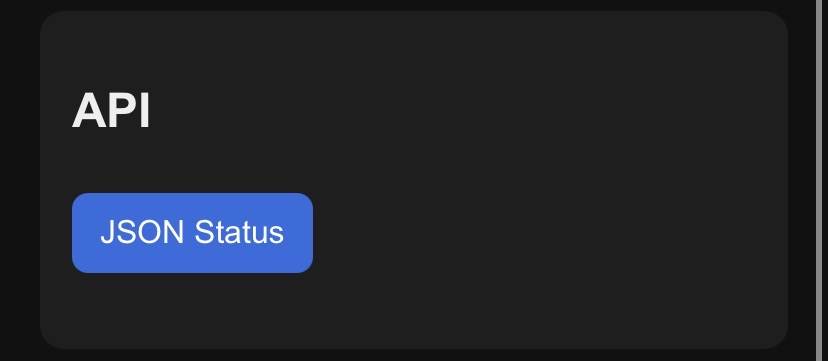
\includegraphics[width=\linewidth]{inhalt/bilder/Json1.png}
      \caption{Segment fünf der \gls{ui}.}
      \label{fig:Json1}
	\end{subfigure}
	\\
	\begin{subfigure}{0.55\textwidth}
      \centering
      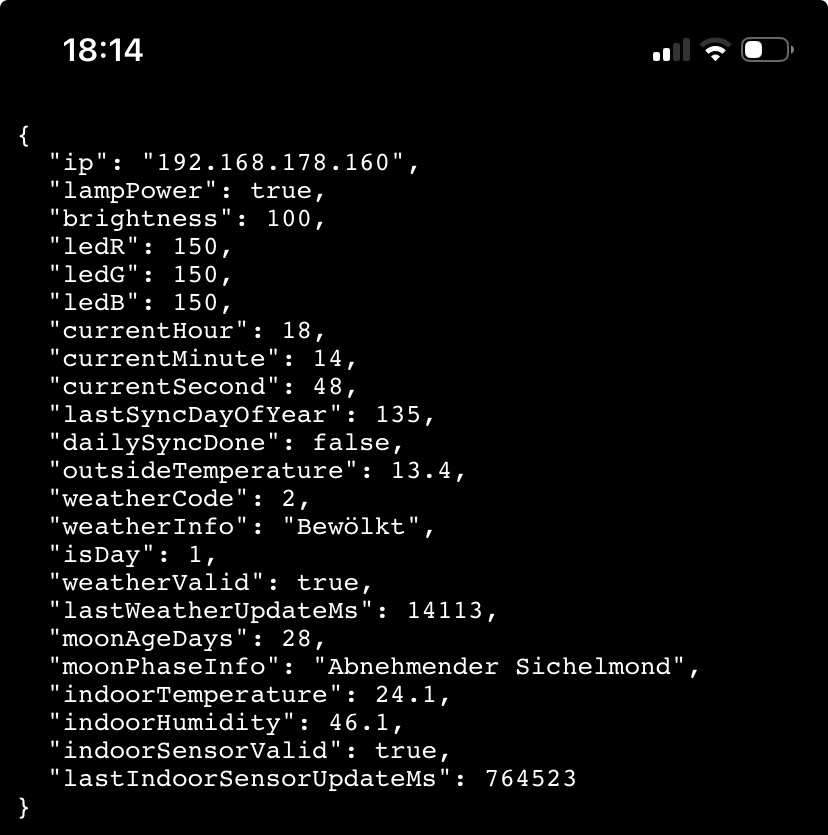
\includegraphics[width=\linewidth]{inhalt/bilder/Json2.png}
      \caption{Das in der \gls{ui} aufgerufene \gls{json}-Statusfile.}
      \label{fig:Json2}
	\end{subfigure}
	\caption{Abruf des \gls{json}-Statusfiles über die \gls{ui}.}
  \label{fig:Json}
\end{figure}